\chapter{Kravspecifikation}\label{ch:Krav}

I projektet er user stories blevet benyttet til at beskrive den ønskede funktionalitet som systemet skal have. Disse stories er lavet på baggrund af MoSCoW-analysen fra afsnit \ref{ch:Moscow}.
De enkelte user stories er blevet samlet til en række af epics, der viser systemets overordnede funktionalitet. Disse epics vises på aktør-kontekst diagrammet, der ses på figur. \ref{fig:KontekstDia}. 

\begin{figure}[H]
	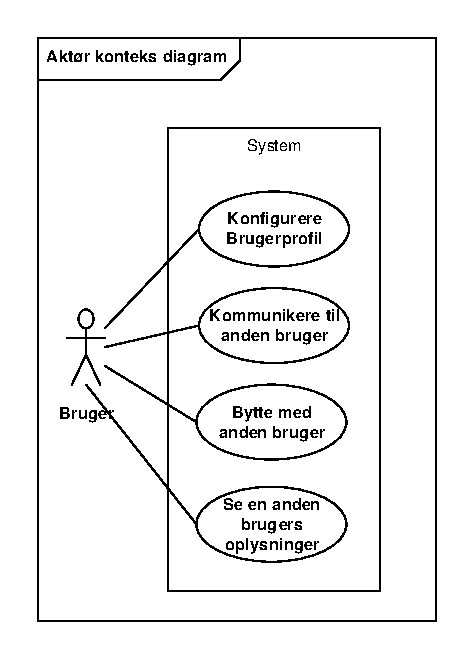
\includegraphics[width=140mm,height=140mm]{../Dokumentation/figures/KontekstDiagram.PDF}
	\caption{Aktør-kontekst diagram for BargainBarter}
	\label{fig:KontekstDia}
\end{figure}

\noindent Igennem rapporten vil der bliver fokuseret på følgende to user stories:''Oprette en bytteannonce'' og ''Søg efter bytteannoncer''. Dette er valgt for at kunne gå i dybden med disse to user stories med hensyn til at redegøre for deres arkitektur, design og implementering. Disse user stories er valgt, da de er blandt de mest centrale for funktionaliteten af systemet. \\ For den fulde liste og beskrivelse af de udarbejde user stories for systemet henvises til dokumentationen \footnote{Se bilag - Dokumentation, sektion 3}\\
De to udvalgte user stories kan læses nedenunder:

\section{Oprette en bytteannonce}
{\color{blue}\textbf{EGENSKAB}:} Oprette en bytteannonce \\
Som bruger \\
Ønsker jeg at kunne oprette en bytteannonce \\
For at kunne bytte med andre brugere af systemet.\\ \\
{\color{blue}\textbf{BAGGRUND}} \\
{\color{blue}\textbf{Givet}} at bruger er logget ind \\ \\
{\color{blue}\textbf{SCENARIE:}} Oprette en bytteannonce \\
{\color{blue}\textbf{Når}}  bruger ønsker at oprette en bytteannonce i systemet \\
{\color{blue}\textbf{Så}} navigerer han til menupunktet ”Opret annonce” \\
{\color{blue}\textbf{Så}} udfylder han bytteannonce-skabelonen \\
{\color{blue}\textbf{Og}} trykker på ”Opret annonce”-knappen
\section{Søg efter bytteannoncer}
{\color{blue}\textbf{EGENSKAB}:}Søg efter bytteannoncer \\
Som bruger \\
Ønsker jeg at kunne søge efter bytteannoncer \\
For at kunne finde en bestemt type vare\\ \\
{\color{blue}\textbf{BAGGRUND}} \\
{\color{blue}\textbf{Givet}} at bruger er logget ind \\
\\
{\color{blue}\textbf{SCENARIE:}} Søg efter bytteannoncer \\
{\color{blue}\textbf{Når}} bruger ønsker at søge efter bytteannoncer i systemet\\
{\color{blue}\textbf{Så}} navigerer brugeren til menupunktet ”Søg” \\
{\color{blue}\textbf{Så}} indtaster brugeren søgekriterier som består af(Kategori, afstand, evt byttegenstand)\\
{\color{blue}\textbf{Og}} trykker på “søg“-knappen

\section{Ikke-Funktionelle krav}
I forbindelse med udarbejdelsen af systemet er der blevet fastsat nogle ikke-funktionelle krav til systemet. De funktionelle-krav omhandler primært performance, brugervenlighed og skalerbarhed. En liste over de ikke-funktionelle krav kan ses nedenunder.
\chapter{Ikke-funktionelle krav}\label{ch:Ikkefunktionelle}

\begin{enumerate}
	\item Man skal kunne komme ind på alle annoncer med kun 2 klik fra forsiden \url{http://10.29.0.30/bargainbarter}
	
	\item Hjemmesiden skal kunne håndtere 10 brugere på samme tid
	
	\item Ved brug af søgefeltet under hjemmesiden skal der maksimalt gå 15 sekunder fra man trykker på ''søg''-knappen før resultaterne er fundet frem og er blevet vist på skærmen
	
	\item Systemet skal have en online hjemmeside (fast IP)
		
	\item Hvis en bruger søger efter en annonceplacering inden for en vis afstand, må den maksimale afstand til den pågældende annonceplacering højst overskride den valgte afstand med 100 meter
	
	\item Hvis bruger A ønsker at kontakte bruger B gennem den indbyggede chat, så skal der maksimalt  gå 10 sekunder fra bruger A trykker ''send'' til, at beskeden afleveret til bruger B
	
	\item Når en bruger ønsker at vurdere en anden bruger, så skal man maksimalt kunne skrive 500 tegn
	
	\item Når en bruger kommenterer en anden brugers annonce, skal der maksimalt gå 15 sekunder fra, at den kommenterende bruger trykker ''Send'' til at den anden bruger kan se kommentaren på den pågældende annonce
	
	\item Hjemmesiden skal kunne tilgås fra følgende enheder (PC, mobil (Android: OnePlus3 og iPhone 5s) og tablet)
	
\end{enumerate}